\documentclass[11pt]{article}

\usepackage[letterpaper,margin=1in]{geometry}
\usepackage[T1]{fontenc}
\usepackage[utf8]{inputenc}
\usepackage{lmodern}
\usepackage{microtype}
\usepackage{setspace} % line spacing
\usepackage{amsmath}
\usepackage{graphicx}
\usepackage{caption}
\usepackage{flafter} % prevent floats from appearing before their definition
\usepackage{titlesec}
\usepackage{enumitem}

% Tight section spacing
\titleformat{\section}{\bfseries\large}{}{0pt}{}
\titlespacing*{\section}{0pt}{0.45\baselineskip}{0.2\baselineskip}

% Tight lists
\setlist[itemize]{nosep,leftmargin=*}
\setlist[enumerate]{nosep,leftmargin=*}

% Captions / floats
\captionsetup{font=small, skip=4pt}
\captionsetup[figure]{labelformat=empty}
\setlength{\textfloatsep}{8pt plus 2pt minus 2pt}
\setlength{\intextsep}{6pt plus 2pt minus 2pt}
\setcounter{topnumber}{1}
\renewcommand{\topfraction}{0.95}
\renewcommand{\textfraction}{0.05}
\renewcommand{\floatpagefraction}{0.9}

% Paragraph / line spacing
\setlength{\parindent}{0pt}
\setlength{\parskip}{4pt}
\setstretch{1.12}
\raggedbottom
\widowpenalty=10000 % never strand a single line across a page break
\clubpenalty=10000

\begin{document}

\begin{titlepage}
\centering
\vspace*{0.3\textheight}
{\Large\bfseries Few-Shot, Joint Embedding Predictive Architectures for Translatable Machine Learning in Biological Preparedness\par}
\vspace{1.8\baselineskip}
{\large SPAR Spring 2027 project proposal
\\ Mentor: William Wang (Yale University, MATS Research)\par}
\end{titlepage}


\section*{Overview}
When a new pathogen appears, natural or engineered, how soon can a model read a patient's molecular state and be trusted in a hospital that contributed no training data? Diagnosis, triage and drug repurposing depend on translational models, ones that still work on a new cohort, a new sequencing platform and a new lab. Most do not. DermTrace is our open collection of more than 1,000 human gene-expression profiles from skin, scar and tumor tissue, evaluated with whole studies held out. It grew out of KeloidBench (Figure 1), whose classifier averages 0.83 macro F1 across held-out studies and scores 0.18 on the worst one. This project builds three ways to close that gap: reinforcement-learning (RL) environments that reward an agent only for results on studies it never saw, JEPA encoders trained on the data we hold, and a zero- and few-shot evaluation that rehearses the first days of an outbreak. The cohort produces a paper and open environments.

\begin{figure}[!ht]
\begin{minipage}[c]{0.56\textwidth}
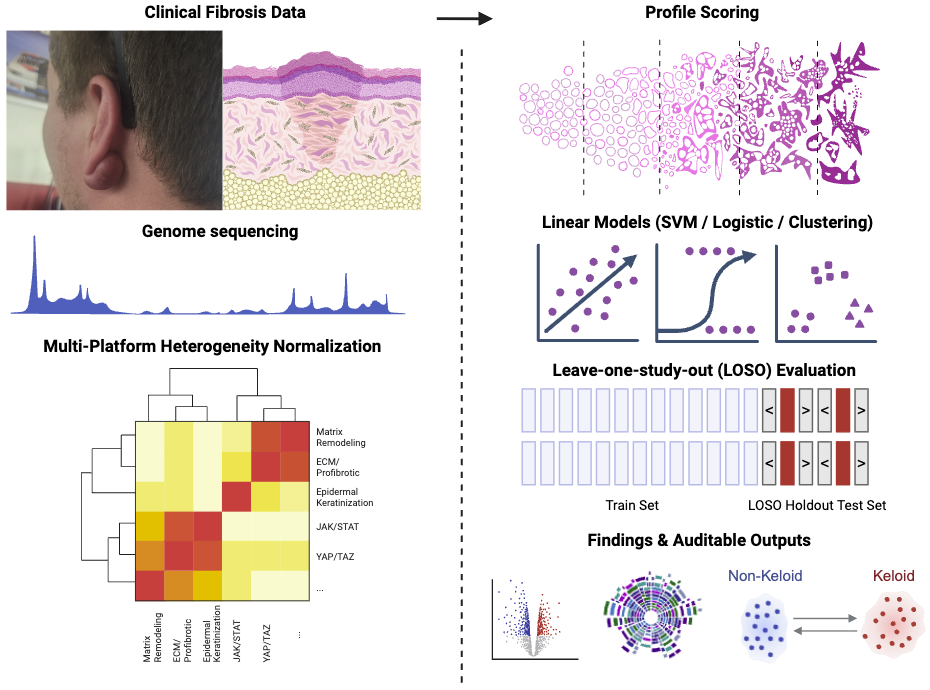
\includegraphics[width=\linewidth]{keloidbench-graphical-abstract.png}
\end{minipage}\hfill
\begin{minipage}[c]{0.4\textwidth}
\caption{\textbf{Figure 1. The starting point.} The KeloidBench pipeline (Wang, Tam and Tsao, NeurIPS GenAI4Health 2026): expression profiles from many platforms are normalized into gene-program scores, classified by linear models, and scored with whole studies held out. The studies each replace a part: (1) agents trained in RL environments build the pipeline; (2) a JEPA encoder replaces the hand-built program scores; (3) the held-out test extends to new cohorts with zero to twenty labels.}
\end{minipage}
\end{figure}

\section*{Why this matters for safety}
\begin{itemize}
\item \textbf{Defense has to work against agents nobody has seen;} as AI lowers the skill needed to modify a pathogen, countermeasures tied to a known one arrive late. The host's response can be read without identifying the pathogen: expression signatures separate bacterial from viral infection across cohorts (Sweeney et al., Sci.\ Transl.\ Med., 2016). Host-directed models are a durable, pathogen-agnostic counter to dual-use threats, but only if they translate.
\item \textbf{Translation is where pandemic ML failed;} a systematic review that screened 2,212 studies of machine learning for COVID-19 imaging found no model fit for clinical use (Roberts et al., Nat.\ Mach.\ Intell., 2021). DermTrace shows the same gap at small scale: a language-model adapter that scored 0.60 in cross-validation fell to 0.32 when whole studies were held out. Targets such as the 100 Days Mission leave no time to learn this after deployment.
\item \textbf{Agents get good at what they are rewarded for;} environments that reward leaderboard fit train agents to overfit faster. Ones that reward held-out performance, sample checks and abstention steer the same capability toward countermeasures that work. Ours hold human host data only: no pathogen sequences, no design tasks and no laboratory work.
\end{itemize}

\section*{Research questions}
\begin{enumerate}
\item \textbf{Can a reward teach translation?} Do agents rewarded on held-out studies build models that hold up on cohorts scored once, compared with agents rewarded on random splits?
\item \textbf{Does latent prediction cross platforms?} Does a JEPA encoder beat masked reconstruction, program scores and a single marker gene when whole studies are held out?
\item \textbf{How few samples are enough?} Given zero, one, five or twenty labeled samples from a new cohort, how accurate and calibrated is each method, and does it abstain when it should?
\end{enumerate}

\section*{Approach}
\textbf{Setting and measurement.} DermTrace holds a 963-profile training corpus from 34 public studies across microarray, bulk and single-cell platforms, plus in-house RNA-seq: 60 samples under four oxygen conditions and 48 archived melanoma tumors, in processing, with mutation status called from RNA. Every result is scored on studies held out whole, lockbox cohorts are scored once under a frozen protocol, and the worst study is reported beside the mean. Each method must beat two baselines: a linear model on program scores and a single gene, COL1A1, which matched it.

\textbf{Three studies}, one per research question, which a team of 1-2 mentees can split:
\begin{enumerate}
\item \textbf{RL environments.} Each environment is a task, a sandbox and a hidden grader. An agent with code tools receives development cohorts and must deliver a model. Its reward is the score on studies it never saw, with terms for calibration and abstention. Task families come from the repository: cross-study classification, transfer of an oxygen-response signature from a cell line to donors, and sample-identity checks whose answers were fixed by SNP genotyping. We fine-tune an open-weight agent under held-out and random-split rewards and score both on the lockbox.
\item \textbf{JEPA encoders.} A JEPA predicts the representation of a masked part of its input, not the raw values (Assran et al., arXiv:2301.08243; for single cells, Cell-JEPA, arXiv:2602.02093). Predicting the embedding of masked gene programs should discard the platform noise that reconstruction has to model. We implement it for bulk and pseudobulk profiles, add a variant that predicts the response to a change in oxygen, and score both under study hold-out.
\item \textbf{Data engineering and the outbreak drill.} New cohorts arrive as they would in an outbreak: unharmonized, from a new platform, with few labels. Mentees extend the pipeline (harmonization, identity checks by genotype, provenance) and score three methods at each number of labels: in-context inference by a language model, a JEPA embedding with a linear classifier, and the program-score baseline. The final lockbox is public host-response cohorts from infection. A first data point exists: of eight hypoxia genes fixed on one cell line, four transferred to 15 donors.
\end{enumerate}

\section*{Possible outcomes}
\begin{itemize}
\item \textbf{Held-out reward changes what agents build.} The environments become open training tasks that steer agents in biology toward results that survive a new cohort.
\item \textbf{JEPA transfers where reconstruction does not.} The paper gives a recipe for encoders at outbreak scale. If one gene still wins, the day-one tool should stay a small marker panel.
\item \textbf{The few-shot curve gives a number.} It says how many labels a new cohort needs before a model can be trusted, and whether skin data can stand in for infection.
\end{itemize}

\end{document}
